\chapter{実験装置の設計\label{devicesection}}
\newpage
\section{概要}
本章では, ファントムに加振した際の1次元的なせん断波の伝播の様子をエコーパルスイメージングおよびリング型アレイトランスデューサ超音波CTで解析することで, ファントムの機械的特性を評価するものである. また, リング型アレイトランスデューサでは現段階ではリアルタイムで生体組織の挙動を観測することはできない. そのため, 各面内で得た断層画像から目的の生体組織を検出する方法についても検討する. また, ファントムの加振した際の挙動を記述する理論式を組み立てることで, 実験値と比較検討する.
\section{加振装置}
\figref{kashinsouchi}は, 本研究で使用した加振装置の概要である. 電圧で駆動させた振動モータを用いてファントムを振動させた. ファントムは弦などのごく細いもので, 一次元的な振動を与えた. 以下では, 加振装置の振動数の設定, ファントムの設定, 張力などの力学的条件の設定, バリデーションについて述べる. 
\begin{figure}[H]
  \begin{center}
    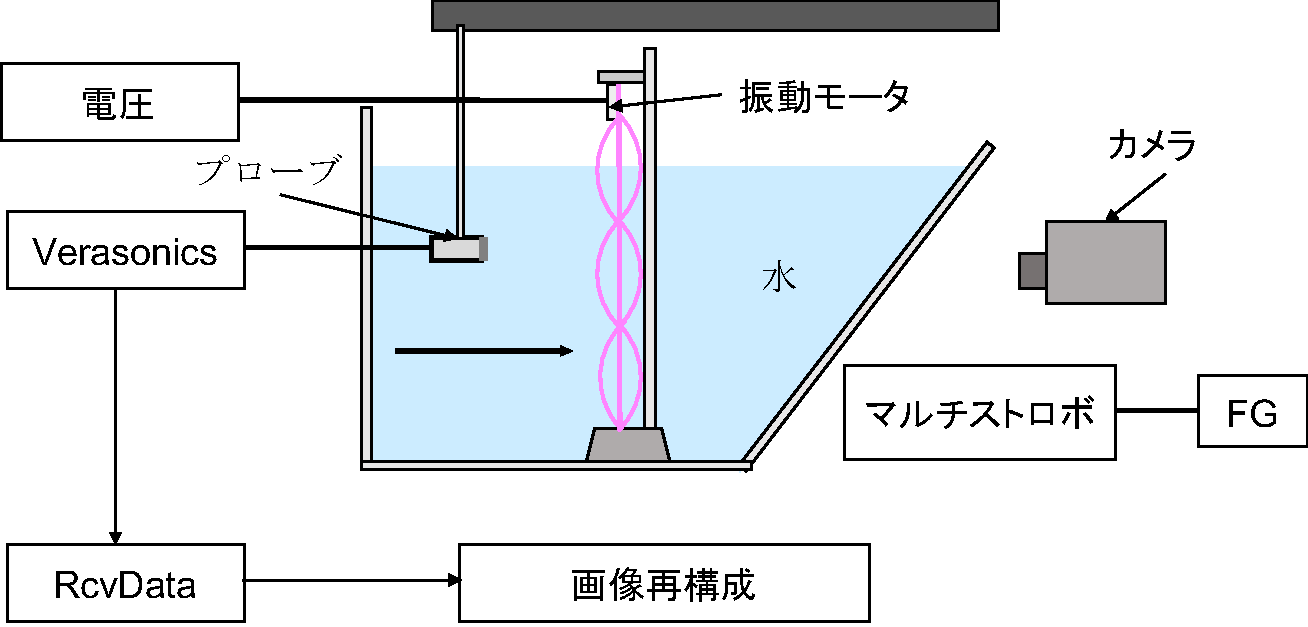
\includegraphics[width=110mm]{fig/jikkendevice.pdf}
  \end{center}
  \caption{加振装置}
  \figlab{kashinsouchi}
\end{figure}
%\begin{itemize}
\subsection{振動数の設定}
生体組織を振動させる方法としては手動, 音響放射圧, 機械的加振がある. その中でも, 機械的加振を選択したのは, 生体組織のより定量的な機械的特性の評価のためである. ファントムの振動手段としては振動モータを使用した. 実際に使用した振動モータを\figref{motor}に示す.
\begin{figure}[H]
  \begin{center}
    \includegraphics[width=70mm]{fig/motor.pdf}
  \end{center}
  \caption{振動モータ}
  \figlab{motor}
\end{figure}
\subsection{ファントムの設定}
本研究では, まずは釣り糸, 水糸のような強度や密度が規格化されているファントムを用いて計測した. その後に鳥の腱を用いて計測することで, 実際の生体組織に関しても本研究の生体組織の特性の定量かの妥当性を検討した. 実際に使用したファントムを\figref{fantom}に示す.
\begin{figure}[H]
  \begin{center}
    \includegraphics[width=30mm]{fig/fantom.pdf}
  \end{center}
  \caption{ファントム}
  \figlab{fantom}
\end{figure}
\subsection{力学的条件の設定}
\subsection{バリデーション}
\begin{figure}[H]
 \begin{minipage}{0.5\hsize}
  \begin{center}
   \includegraphics[width=40mm]{fig/led.pdf}
  \end{center}
  \caption{LED}
   \figlab{led}
 \end{minipage}
 \begin{minipage}{0.5\hsize}
 \begin{center}
  \includegraphics[width=70mm]{fig/fanction.pdf}
 \end{center}
  \caption{ファンクションジェネレータ }
  \figlab{fanction}
 \end{minipage}
\end{figure}
%\end{itemize}